
%------------------------------------------------------------------------------
%                        Paper document class & title
%------------------------------------------------------------------------------


\RequirePackage{fix-cm}
%\documentclass[10pt]{sig-alternate-05-2015}
\documentclass[10pt, conference, letterpaper]{IEEEtran}

\def\flowqos{\textsc{FlowQoS}\xspace}
\def\papertitle{{\fontsize{20.74}{12}\bf\scshape \flowqos}: Not Every Flow is Born
the Same}
\def\pdfauthors{}
\def\paperkeywords{}


%------------------------------------------------------------------------------
%                                Pre-package misc.
%------------------------------------------------------------------------------

\usepackage{xcolor}

% Link colors
\definecolor{linkcol}{rgb}{0,0,1}
\definecolor{citecol}{rgb}{0,0.5,0}
\definecolor{urlcol}{rgb}{0.3,0,0}

% Set PDF is paper dimensions to be Letter size.
\setlength{\pdfpagewidth}{8.5in}
\setlength{\pdfpageheight}{11in}


%------------------------------------------------------------------------------
%                                Use packages.
%------------------------------------------------------------------------------

\usepackage[normalem]{ulem}
\usepackage{tikz}
\usepackage{amsmath}
\usepackage{ragged2e}
\usepackage{cite}
\usepackage{txfonts}
\usepackage{fancyhdr}
\usepackage{amssymb}
\usepackage{fancyvrb}
\usepackage{graphicx}
\usepackage{times}
\usepackage{pifont}
\usepackage{url}
\usepackage{xspace}
\usepackage{epstopdf}

\usepackage[aboveskip=5pt,small,labelfont=bf]{caption}
\usepackage{subcaption}

\usepackage[bookmarks=true,%
bookmarksnumbered=true,%
colorlinks=true,%
linkcolor=linkcol,%
citecolor=citecol,%
urlcolor=urlcol,%
hypertexnames=true,%
pdfpagelabels]{hyperref}

\usepackage{multirow}


%------------------------------------------------------------------------------
%                                Space savers.
%------------------------------------------------------------------------------

\setlength\floatsep{5pt}
\setlength\textfloatsep{10pt}
\setlength\intextsep{5pt}

\makeatletter
\def\url@myurlstyle{%
   \@ifundefined{selectfont}{\def\UrlFont{\small}}{\def\UrlFont{\small}}}
   \makeatother
\urlstyle{myurl}


%------------------------------------------------------------------------------
%                                Misc.
%------------------------------------------------------------------------------

% This adds ':' to the characters after which not to break URLs, and
% defines a smaller typewriter font. --cpk
% changed small to sf -- md
\def\UrlNoBreaks{\do:\do\(\do\[\do\{\do\<}%
\def\UrlFont{\small\ttfamily}
\def\UrlOrds{\do\*\do\~}%

% For referencing sections, Vern-style
\newcommand\xref[1]{\S~\ref{#1}}

\newcommand\fref[1]{Fig.~\ref{#1}}


%------------------------------------------------------------------------------
%                                New commands
%------------------------------------------------------------------------------

% For notes to other authors:
\newcommand{\note}[1]{{\textcolor{red}{\textit{#1}}}}
\newcommand{\ignore}[1]{{\textcolor{red}{\sout{\textit{#1}}}}}


\newcommand{\code}[1]{\texttt{\small{#1}}}
\newcommand{\mycomment}[1]{}
\newcommand{\todo}[1]{\textbf{TODO: #1}}
\newcommand{\mytab}{~~~~}
\newcommand{\sspace}{~}
\newcommand{\etal}{\textit{et al.}}
\newcommand{\eg}{{e.g.,}}
\newcommand{\ie}{{i.e.,}}
\newcommand{\lno}[1]{{\tiny{\textbf{(#1)~~}}}}
\newcommand{\toolx}[1]{{\fontsize{#1}{12}\bf\scshape \tool}}

\newcommand{\of}{OpenFlow}
\newcommand{\rulesep}{\unskip\ \vrule\ }
\newcommand{\sdn}{{SDN}}
\newcommand{\ltc}{{Linux Traffic Control}}
\newcommand{\ovs}{{OpenvSwitch}}
\newcommand{\htb}{{HTB}}

\renewcommand{\thetable}{\arabic{table}}

% \newcommand*{\refname}{Bibliography}

\hypersetup{
pdfauthor = {},
pdftitle = {\papertitle},
pdfkeywords = {\paperkeywords},
pdfcreator = {LaTeX with hyperref package},
pdfproducer = {pdflatex}}

\begin{document}
 
\title{\papertitle}


\author{\IEEEauthorblockN{Dhruv Sharma}
\IEEEauthorblockA{UC San Diego, CA\\
dhsharma@cs.ucsd.edu}
\and
\IEEEauthorblockN{Robert Jenkins}
\IEEEauthorblockA{UC San Diego, CA\\
rfjenkins@ucsd.edu}
\and
\IEEEauthorblockN{Frederik Nygaard}
\IEEEauthorblockA{UC San Diego, CA\\
freddyny@ucsd.edu}
\and
\IEEEauthorblockN{Feichao Qian}
\IEEEauthorblockA{UC San Diego, CA\\
feqian@ucsd.edu}}


\maketitle

\begin{abstract}
%%
{
% \small
% 
With majority of the world's data and computation handled by cloud-based
systems, cloud management stacks such as Apache's CloudStack, VMware's vSphere
and OpenStack have become an increasingly important component in cloud software.
However, like every other complex distributed system, these cloud stacks are
susceptible to faults, whose root cause is often hard to diagnose. We present
Hansel, a system that leverages non-intrusive network monitoring to expedite root
cause analysis of such faults manifesting in OpenStack operations. Hansel is fast and
accurate, and precise even under conditions of stress.
}
%%
\end{abstract}

\section{Introduction}
\label{sec:introduction}

%why we need FlowQos?
In modern times, user devices connected to broadband access networks, run an assortment of applications that exchange network traffic with remote servers and other devices over the Internet. Since the upstream and downstream throughput is generally limited, these traffics will compete for relatively scarce bandwidth resources. 

However, traffic from one application might not share the same characteristics as the traffic created from another application. To a large extent, it is the end-user’s requirements that play a significant role in deciding the nature of such applications and hence the kind of network traffic they send and receive. For instance, a user’s expectation from a VoIP call, video streaming and gaming applications is that their experience remains seamless and high quality during their use of the application, requiring the traffic to be sent out at near constant rates with low delay and high reliability paths over the network. Whereas, in certain use cases such as data backup to the cloud and system updates, it is expected that the operation is completed eventually- even when the user is not actively using the application. Traffic from such applications, in contrast to VoIP and video streaming, does not come with any hard deadlines or network requirements.

While the nature of traffic varies so widely, the network devices today are, to a large extent, agnostic to such subtleties in the nature of network traffic and tend to handle it in the same way. Even though later kinds of applications discussed above do not face any issues that directly affect the user, the former kind might be impacted severely due to the effect on network dynamics leaving the user with a sour experience. 

%previous work
Research over the past years has resulted in the use of various metrics such as packet delays, jitter, available bandwidth, frame rate etc. to quantify user’s experience in some way. One possible way to deal limited throughput is to configure the network routers to prioritize some specific applications' traffic flows (e.g. video, VoIP etc) over others (e.g. data backup, file upload etc). It will effectively improve Quality of Service (QoS). However, for some reason, previous work on QoS mechanisms have not been deployed in broadband access networks~\cite{Seddiki2014}. The emergence of software-defined networking (SDN) gives more possibilities to solve this problem. One approach to deploying QoS in broadband access networks is to utilize the advantages of SDN that separates the network's control logic and forwarding planes. We can migrate the functions that perform QoS both application identification and router-level configuration to separate control logic, and design a front-end client (e.g., webpage) at high levels of abstraction to let users to assign bandwidth to each identified application according to their own preference. Once users set up their preference, the front-end will install the QoS configuration into the home routers~\cite{Seddiki2014}. This approach makes it easy for user to configure priorities and facilitates more sophisticated per-flow application based QoS. 

%Our solution
\subsection{Our Solution}
In this paper, we focus on FlowQoS~\cite{Seddiki2014} solution that utilizes SDN and traffic policing in virtual switches to achieve network isolation in traffic flow types. We further provide an alternate implementation using Linux traffic control features to achieve the same goal with optimizations in the use of available bandwidth.

%Our contribution
\subsection{Our contributions}
First, we deploy the FlowQoS implementation of pair of virtual switches for improving QoS, within a virtual machine (emulating our end-host) with Internet connection instead of the discussed hardware implementation. Second, we validate the results presented by FlowQoS~\cite{Seddiki2014} using similar tools and scenarios that they used. Finally, we intend to develop an SDN controller and agent application that utilizes Linux’s advanced routing and traffic control to implement the idea of FlowQoS while overcoming the limitation of under-utilization of available bandwidth. 

%The rest of the paper
\subsection{Outline}
{\color{red} Need to be modified.} The rest of the paper is organized in the following way: We discussed related work in QoS, as well as SDN-based solutions for home and broadband access networks in section \rom{2}. The motivation of FlowQos is presented in Section \rom{3}. Section \rom{4} records some problems we encountered. Section \rom{5} describes the design of FlowQoS and Section \rom{6} describes its implementation. Section \rom{7} evaluates FlowQoS for video streaming and VoIP applications in the context of competing flows. We discusses future work and open research avenues in Section \rom{8} and concludes in Section \rom{9}.


\section{Related Works}
\label{sec:related-works}

\section{Motivation}
\label{sec:motivation}
Congestion has been, and continues to be, one of the most prevalent problems in networking.  One of the key issues with TCP is that when there are many flows it has a tendency to cause congestion, leading to degraded performance of competing flows.  This degradation can range in cost from minimal to disastrous.  When TCP connections consume all the available bandwidth real-time applications have a tendency to suffer the most. This is true because real-time applications have tighter latency and throughput constraints.

Our motivation for exploring FlowQoS is to provide better quality streaming services, which cannot afford to compete with flows like TCP which can dominate them.  It is commonplace for many users to have multiple web pages with active web traffic while simultaneously using a streaming service like Skype or VoIP- we believe that flow classification described in FlowQoS can prevent these users from receiving poor Skype call quality due to congestion that they may be creating.

One of the downsides of FlowQoS is that it statically allocates bandwidth to classes of traffic, such as TCP or UDP.  This is detrimental to throughput when certain classes are not fully utilizing their allotted bandwidth.  By using the concept of classifying traffic from FlowQoS and dynamically allocating bandwidth we will show that we can still achieve get the target quality of service that FlowQoS provides, while providing a total throughput that is closer to a non-regulated network.
% \input{sections/goals.tex}
\input{sections/problem.tex}
\section{Design}
\label{sec:design}

The original FlowQoS prototype was implemented on Raspberry Pi running OpenWrt Linux distribution with Openvswitch integration. However, since the aim of this paper is to validate the claims and results that demonstrate the need for FlowQoS-like systems rather than its deployment feasibility, we implement our solution within the virtual networking environment in end-host Linux distribution. Though such implementation can be still be easily moved to a dedicated device.

\begin{figure}[t]
\centering
\includegraphics[width=0.9\linewidth]{architecture}
\caption{FlowQoS architecture.}
\label{fig:architecture}
\end{figure}

The FlowQoS's OVS-based architecture (~\fref{fig:architecture}) is comprised of dual-OVS topology with multiple paths between them passing through "dumb" forwarding bridges. Each path between the two OVSes (\texttt{ovs-in} and \texttt{ovs-out}) corresponds to a high-level traffic class to which the user or administrator wishes to classify any ingress (or egress) traffic to (or from) the end-host. Both \texttt{ovs-in} and \texttt{ovs-out} are configured to run in secure Openflow mode such that the OVS would accept Openflow commands from the Openflow controller when connected to it and in its absence it would not default to learning switch mode. This is required to prevent the runaway issue in learning switch network topologies with cycles. The physical interface (\texttt{eth0} in our case) connecting the end-host to the physical network is attached to \texttt{ovs-out}, whereas, the IP address for the end-host machine is moved from \texttt{eth0} to the virtual ethernet interface \texttt{veth0}. Such a setup ensures that any traffic from any application must traverse dual-OVS virtual topology before leaving the end-host and vice-versa for the incoming traffic. While the connecting bridges between \texttt{ovs-in} and \texttt{ovs-out} provide no functionality of their own, we use them solely for packet capture and debugging purposes.

In our implementation of HTB-based architecture, we combined \texttt{ovs-in} and \texttt{ovs-out} in ~\fref{fig:architecture} into one OVS and enable an HTB qdisc (queueing discipline) on \texttt{veth0} and \texttt{veth1}. To this qdisc, we added one parent class and four leaf classes each for one traffic type. The leaf classes are: \textbf{Video}, \textbf{VoIP}, \textbf{Gaming} and \textbf{Web}. To this, we added filters to classify the different traffic types and finally assign priorities to the each sub-class such that \textbf{Video} and \textbf{VoIP} get the highest priorities followed by \textbf{Web} traffic and finally the \textbf{Gaming} (unclassified) traffic gets the least priority.

We now discuss the two primary components of the FlowQoS controller module - namely, the Flow Classifier and the Rate Controller.

\subsection{Flow Classifier}
FlowQoS's classifier is comprised of two sub-modules - HTTP classifier and non-HTTP classifier. The reason for such initlal segregation is that modern HTTP applications no longer just carry textual web traffic but can include embedded components such as video players, advertisements, images etc. each generating traffic of different nature.
Therefore, identifying traffic to be HTTP is not sufficient and further analysis must be done to ascertain the type of traffic that the HTTP stream is actually carrying. Hence, any incoming packets from underlying Openflow layer are categorized HTTP (or HTTPS) based on the source or destination port being 80 (or 443).

With this goal in mind, FlowQoS was designed to inspect DNS queries that an HTTP application makes before it even sends or receives any HTTP traffic. The classifier uses a preconfigured list of DNS CNAME records to match a domain to its application type. The list is continuously updated based on the expiry time of DNS record. Hence, when an HTTP traffic has source or destination that matches the regular expression for that domain, it is classified based on the pre-identified traffic type.

On the other hand, for non-HTTP traffic, FlowQoS makes use of the \texttt{libprotoident} \cite{flow_web} library. The library requires certain additional information to be captured from the packets apart from the protocol type, source destination IP addresses and ports. Particularly, it uses the first 4 payload bytes and payload size for the first packet in either direction flows of a connection (or just one direction in case of unidirectional flows).

However, our initial exprimentation with applications we use to evaluate FlowQoS did not result in correct identification of the protocol due to multiple reasons such as unavailability of DNS resolution for locally hosted HTTP server and due to certain protocols (eg. Skype and Iperf TCP) not showing specific packet signature for classification by \texttt{libprotoident} library. Therefore, for our evaluation we fall back to the default port-based protocol identification technique.

\subsection{Rate Controller}
FlowQoS's rate controller hosts REST APIs to receive a bandwidth distribution from the user and generate a parsable JSON configuration file to used on the end-host to enforce rate limits on each kind of traffic.
Since, the primary focus of this paper is not to validate the accuracy of the flow classification, but rather the effectiveness of classification and rate limiting in improving application performance, we now evaluate the two different schemes of enforcing rate limits along with their pros and cons based on the evaluations with various traffic types in ~\xref{sec:evaluation}.

\section{Background}
\label{sec:background}

Before we discuss FlowQoS's overall design we would like to introduce the concept of traffic policing and traffic shaping. While both techniques can be used for effectively limiting the rate at which traffic is forwarded through a link, these fundamentally differ in the way they handle the network packets.

Traffic policing is usually implemented using token-based approach where based on the set rate limit, a fixed number of tokens are allocated to an interface at the end of each token refresh period. As packets of corresponding sizes are forwarded the token count is reduced until no more tokens can be removed. This ensures that the interface does not send traffic more than the stipulated rate. However, if there are still packets left with the interface that could not be sent, the policer simply drops those packets. Also due to token based nature of policer, packet bursts get forwarded by the interface. The OpenvSwitch (OVS) ~\cite{ovs} implements rate limiting using traffic policing that is used by the FlowQoS's original architecture.

Traffic shaping, on the other hand, is implemented using a leaky-bucket approach (one variant of this is equivalent to a token-based approach) which in fact calculate an equivalent rate metric based on system architecture timer resolution and forwards traffic continuously strictly conforming to this rate. Any burst pf packets (packets at higher rate) are buffered in a short internal queue and delayed until the shaper acheives the desired transmission rate. Only when the queue becomes full, the residual packets are dropped. Due to this queuing, packets are expected slightly higher latencies than normal. The Hierarchical Token Bucket (HTB)~\cite{htb_manual} queuing discipline provided by the Linux's traffic control suite implements traffic shaping that follows a similar approach to forward traffic.

\begin{figure}[t]
\centering
\includegraphics[width=0.9\linewidth]{LTC}
\caption{HTB Hierachical Class Structure Illustration.}
\label{fig:htb}
\end{figure}

Moreover, HTB is classful queuing discipline that allows adding multiple traffic filter (classes) under the root filter (class), which can further have sub-filters (sub-classes) forming a traffic classification tree. Each of the intermediate and leaf classes can have individual rate limits and therefore traffic shapers associated with them. In addition, they also have an associated priority that is respected by HTB while sharing unutilized bandwidth among multiple sibling classes. ~\fref{fig:htb} illustrates such a heirarchical structure described above and shows how egress traffic is partitioned into multiple classes.\\

%OVS and HTB both helps you to control a given link's outbound bandwidth. HTB is a quick, intuitive qdisc which is meant to be more understandable. It can send different kind of traffic on different links. To do this, we have to decide which link to use when a given packet is going to be sent.

%HTB can ensure that a service is provided with at least the minimum it requested by setting the rate on that class. If a class uses less than the rate it requested, the remaining bandwidth is being used by the other classes who needs more bandwidth. This is called borrowed bandwidth, and prioritizing decide who gets more bandwidth. 

%HTB decides how the bandwidth is being shared by comparing priorities. As we saw in OVS, only the rates are being considered. However, this could give bad utilization if a link uses less bandwidth than it initially is assigned to. 

%In HTB on the other hand, we use the borrowed bandwidth to exploit the unused bandwidth. Therefore, we are also able to assign the maximum bandwidth a class need. We do this by setting the ceiling-value for a class. The priorities of the classes and filters decides which class/qdisc get the available extra bandwidth.

%In HTB we use filters to classify the traffic when it enters a classful qdisc. To decide which class the packets should go to, we consult the filters. The filters attached to the classful qdisc return a decision to the qdisc. The qdisc then uses the decision to decide which class it should send the packet to.
%needs to be redone
%Prioritization of traffic has two crucial elements. First, it needs to tell how the excess bandwidth are distributed amongst siblings as mentioned above. HTB assigns excess bandwidth to the highest priority classes first. However, this allocation must consider the ceiling and rate rules which should always be followed. Second, when you prioritize one class to get less delay, the other classes will always have worse delay because of this. Therefore, when you prioritize packets, it's important to both consider the rate you give the class you prioritize, so you do not kill the other links.




%On figure \fref{figure:htb}, you can see a typical HTB-structure. Each class can have subclasses and filters. Here root class 1:0 is parent to class 1:10 and 1:20. The subclasses should have the same rate combined as their parent, and their ceiling should not go above their parents rate. 



\section{Evaluation}
\label{sec:evaluation}


\begin{figure}[t]
    \includegraphics[width=0.9\linewidth]{dash_max_latencies}
    \caption{Reduction in maximum segment latencies with DASH streaming using FlowQoS's OVS-based architecture}
    \centering
    \label{fig:dash_max}
\end{figure}
 
\begin{figure}[t]
    \includegraphics[width=0.9\linewidth]{dash_frame_drops}
    \caption{Reduction in number of frames dropped with DASH streaming using FlowQoS's OVS-based architecture}
    \centering
    \label{fig:dash_frame}
\end{figure}

In this section, we evaluate the effectiveness of multi-channel OpenvSwitch design in improving the performances of namely three audio-video streaming applications. Each of these applications produce delay and loss-sensitive video traffic. However, the sensitivity to these factors varies differently for these applications and hence the metrics to measure user-satisfaction are also different for each of these applications.

In addition, we evaluate and discuss the improvements that our proposed hierarchical token bucket (HTB) design can bring by replacing the OVS-based scheme while performing the similar classification and rate-limiting functionality as before.

Now, we discuss the three applications that we used to for our evaluation and discuss their results. For each application we measure the corresponding performance metrics under the following three scenarios:-

\begin{itemize}
\item The application alone sends (or receives) traffic and gets maximum available bandwidth.
\item The application competes for bandwidth with a heavy, long-running TCP-based background traffic in the absence of FlowQoS scheme.
\item The application and the heavy, long-running TCP-based background traffic share 50\% of the maximum available bandwidth each by employing FlowQoS's classification and rate-limiting scheme.
\end{itemize}

To emulate a real-life TCP-based background traffic we used the Iperf utility ~\cite{iperf} available in all major Linux distributions. The utility is used to measure TCP or UDP throughput and can run in both client and server mode depending on the command-line arguments. As a server it accepts connections at specified port and receives high amounts traffic on that connection, whereas as a client it connects to specified server address and sends high amount of TCP or specified amount of UDP traffic to the Iperf server.

\subsection{FlowQoS with OVS-based architecture}

\subsubsection{DASH-JS Player}
\label{sec:evaluation:dash-js-player}
The Dynamic Adaptive Streaming over HTTP (DASH) \cite{Dash} is an adaptive bitrate-based video streaming technique where a large video file is partitioned into small segments worth few seconds (or minutes) of playback time and each segment is encoded in multiple bitrates and stored at the streaming server. The segments are sent as HTTP responses to the video player in end-host's web browser where it is decoded and played. In conditions of congestion or packet loss, DASH-JS player \cite{Dash} reduces the bitrate requirements and the streaming server starts streaming the subsequent segments at a lower bitrate.

While the original paper, discusses the effectiveness of their scheme on adaptive bitrate and throughput, we evaluate two other important metrics critical to user experience - the segment arrival latency and number of frames
dropped. High segment arrival latencies tend to cause low buffer lengths at the video player leading to the video playback freezing frequently. Whereas, the number of dropped frames indicate that even though some initially dropped packets were re-transmitted by underlying TCP layer in HTTP, they did not reach the buffer in time for playback and the were dropped. For a user's perspective, this causes the video to suddenly jump ahead (sometimes giving the experience popularly known as "robotic movements") during playback.

The results were collected by setting up two VMs running Ubuntu.  One of the VMs acted as a client requesting the video data and hosting an iperf server.  The other VM acted as the server, sending the video data as well as running 16 iperf processes to fill up the bandwidth and cause network congestion.
Figure \ref{fig:dash_max} shows the max latencies of the segments as they are being streamed from the server VM to the end-host VM.  Streaming without flow classification has the largest range of values, and indeed exhibited the worst experience for watching the video.  After adding the flow classifier, not only did the streaming perform better, but there was significantly less variation- almost comparable to having no traffic.

The best measure of how these results affect user experience is perhaps in the number of dropped frames. Figure \ref{fig:dash_frame} shows that flow classification with background traffic is able to outperform the same scenario without flow classification. This result corroborates the work from the FlowQoS paper that flow classification can be used to prioritize traffic types to give the best user-experience.

\subsubsection{VLC Real-time Streaming}
\label{sec:evaluation:vlc-rtp-streaming}
The VLC media player \cite{vlc} is a portable, free and open-source cross-paltform media player and streaming media server developed as a part of the VideoLAN \cite{vlc} project. For our evaluation we used a VLC server-client player to stream the Big-Buck-Bunny video (often used to compare multiple video standards, encoding schemes and protocols) over a private network using the Real-time Transport Protocol (RTP) \cite{rtp} with MPEG encoding. Unlike DASH, VLC's video streaming server uses UDP as transport protocol for RTP, sends data in single encoding format and maintains a small playback buffer. Therefore, during congestion, it suffers higher frame drops compared to DASH due to UDP packet loss and small playback buffer size. Also, due to single encoding format, the server cannot vary the bitrate to adjust reduce the packet loss suffered during the streaming leading to poor quality video for its complete playback time.

\begin{figure}[t]
    \includegraphics[width=0.9\linewidth]{vlc_ovs.pdf}
    \caption{Improved VLC (RTP) video streaming bitrate with FlowQoS's OVS-based architecture.}
    \centering
    \label{fig:vlc_ovs}
\end{figure}

%\note{[Explain VLC experiments and results here.]}
For evaluating the impact of FlowQoS on the RTP-based stream performance, our setup was similar to the experiment for DASH-JS player. We had two VMs, one for end-host running VLC RTP client and Iperf TCP server, and the other VM running VLC RTP server and Iperf TCP client such that we have high amount of both RTP and regular TCP traffic coming in to the end-host VM. ~\fref{fig:vlc_ovs} shows bitrate variation for the three scenarios we described in ~\xref{sec:evaluation}.
Clearly, bitrate for RTP stream is lower when it has to compete with the TCP stream for bandwidth. However, FlowQoS based traffic isolation actually helps us achieve a bitrate values equivalent to the case where RTP has no competing traffic. While it only seems to be a ~100Kbps of bitrate difference, the video quality from a user's perspective is incredibly poor when FlowQoS is not used for flow isolation leading to large sections of video screen being blacked-out.

\subsubsection{Skype}
\label{sec:evaluation:skype}

Skype \cite{skype} is a popular Voice over IP (VoIP) service, recently acquired by Microsoft, that provides real-time audio, video calling and text messaging functionality using a closed source proprietary protocol running over the network (IP) layer. Currently, it forwards the video (and audio) traffic between two clients via an hybrid peer-to-peer overlay of Microsoft super-nodes spread across the globe.

Compared to DASH and RTP-based video streaming, the quality and real-time constraints on Skype video calls are much harder requiring high stability in the birates and packet interarrival times to keep interaction between two individuals as seamless as possible. Therefore, we take the variation in packet interarrival times at the client side as a measure of performance for FlowQoS implementation. This measure is often known as \say{jitter} and is measured in units of time (usually milliseconds). Skype clients often come with a feature to enable real-time in-call statistics reporting jitter, round-trip time (RTT), capture frame rate, bitrate etc. We use the jitter values reported by Skype's in-call statistics.

However, to ensure that minor network variations do not vary jitter values significantly, we chose to conduct a long distance international video call that ensured relatively stable jitter and RTT values with Skype traffic alone, and we simultaneously monitored for changes in the relay path that could affect these measures.

\begin{figure}[t]
    \includegraphics[width=0.9\linewidth]{skype_call_ovs.pdf}
    \caption{Reduced Skype Video Call Jitter with FlowQoS's OVS-based architecture.}
    \centering
    \label{fig:skype_ovs}
\end{figure}

%\note{[Explain Skype experiments and results here.]}
Unlike, the cases with DASH-JS player and VLC video streaming, Skype requires Internet access. Hence, for this experiment we used one VM as the end-host running Skype client as well as a \textit{wget} \cite{wget} utility as the FTP client downloading a large OS image from a remote FTP server. As shown in ~\fref{fig:skype_ovs}, we observed that both Skype's UDP traffic competes with the incoming FTP (TCP) traffic, the jitter for the Skype call is not only high on an average but it also varies drastically over time. On the other hand, using FlowQoS's OVS-based isolation scheme we could achieve lower and more stable jitter values. The result show with FlowQoS we can achieve even lower jitter compared to the case where Skype is run standalone. We believe such a result can be attributed to the variation in network conditions as well as effect of queuing in FlowQoS OVSes, though further investigation might be required to validate this claim.


\subsection{FlowQoS with HTB-based Architecture}
\label{sec:evaluation:htb}

\subsubsection{Efficient Bandwidth Utilization}

\begin{figure}[t]
    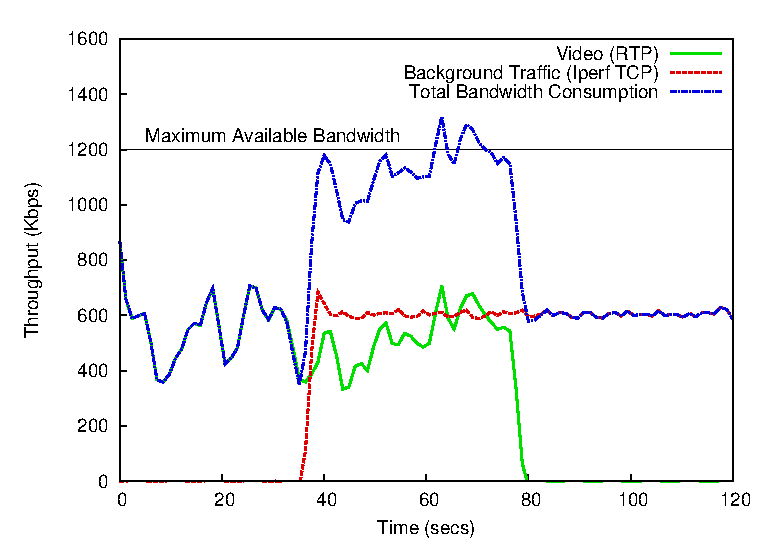
\includegraphics[width=0.9\linewidth]{plot_inefficient}
    \caption{Inefficient Bandwidth Utilization with FlowQoS's OVS-based architecture.}
    \centering
    \label{fig:inefficient_bandwidth}
\end{figure}


\begin{figure}[t]
    \includegraphics[width=0.9\linewidth]{plot_efficient}
    \caption{Efficient Bandwidth Utilization with FlowQoS's HTB-based architecture.}
    \centering
    \label{fig:efficient_bandwidth}
\end{figure}

While, the results with the FlowQoS's OVS-based architecture were impressive, it still suffers from a significant drawback of under-utilizing the network bandwidth in the absence of any competing higher priority traffic. ~\fref{fig:inefficient_bandwidth} shows such a scenario. From 0-40 secs interval, video traffic gets the complete bandwidth for it's use. Between 40-80 secs interval, a competing Iperf TCP traffic runs in parallel getting 50\% of the bandiwdth share. However, during the 80-120 secs interval, the video traffic (high priority) has stopped but the TCP still gets 50\% bandwidth share leading to a 50\% wastage of available bandwidth.

In comparison, by using a Hierarchical Token Bucket approach, the ceiling rate and priority values for each HTB traffic can be configured to enable a high priority class to share it's unused bandwidth with an immediate lower priority class. ~\fref{fig:efficient_bandwidth} shows a similar scenario we saw earlier, however, we can clearly observe that during 80-120 secs interval, the absence of video traffic gives the total available bandwidth to the lower priority TCP traffic. This leads to an efficient utilization of available bandwidth compared to the OVS-based solution.



\subsubsection{DASH-JS Video Player}

\begin{figure}[t]
    \includegraphics[width=0.9\linewidth]{dash_mean_latencies}
    \caption{Reduction in mean latencies for classified flows using FlowQoS's HTB architecture}
    \centering
    \label{fig:dash_mean}
\end{figure}

We re-experimented with the DASH-JS video player on a similar server-client setup as before, but used FlowQoS's HTB-based architecture instead. We observed that not only the average segment latencies decreased for the scenarios in which video traffic was isolated but also observed that the overall variation (measured by the standard deviation) in the latencies also reduced. This can be attributed to the fact that in either case video traffic does not saturated its class's bandwidth share and therefore, HTB did not require to buffer any packets and forwarded a continous stream immediately, whereas due to the relative simplicity of the OVS rate-limiting implementation, it is less accurate in rate estimation and handling fragmented packets leading to higher latencies.
Also, we see that for the case where both video traffic compete, HTB architecture gives higher latencies. We attribute this to the fact that such a situation leads to congestion on that link causing buffering in HTB's traffic shaper that adds queuing delays to the packets. Whereas in case of OVS's policing, such packets are dropped and since DASH-JS player only reports latencies for segments received, OVS seems to perform better even though it would see higher packet loss rate.

\subsubsection{VLC Video Streaming}

\begin{figure}[t]
    \includegraphics[width=0.9\linewidth]{vlc_ltc}
    \caption{Improved overall bitrate for unclassified flows using FlowQoS's HTB architecture}
    \centering
    \label{fig:vlc_ltc}
\end{figure}

We repeated the three scenarios mentioned in \xref{sec:evaluation} with the FlowQoS's HTB-based architecture in place for VLC-based video streaming experiment as shown in \fref{fig:vlc_ltc}. We observed that HTB-based approach indeed produces bitrates equivalent to the OVS-based architecture when we classify and isolate traffic along multiple paths. Moreover, it also improves the overall bitrate of the VLC video streaming even when we do not isolate it from TCP traffic. This can be attributed to the traffic shaping nature of HTB due to which it prefers delaying packets rather than dropping them leading to a higher overall bitrate. Eventhough, this leads to high variation in the bitrate over time, we observed that due an overall increase in mean bitrate user experiences a relatively good video quality.\\\\
\section{Discussion \& Future Work}
\label{sec:discussion}
Through our experiments, we observed that the FlowQoS architecture in either case helps in increasing the overall bitrate for VLC-based RTP video streaming, reduces overall jitter for Skype video calls and reduces the overall segment latencies in comparison to the scenario where both of must compete for their share of bandwidths.
Moreover, we observed that our alternate implementation of the FlowQoS architecture using HTB queuing routine certainly improves bitrate for video traffic when it competes with a simultaneous TCP traffic, reduces latencies for DASH-JS segment delivery and provides a much more efficient utilization of available bandwidth by a lower priority traffic in case a higher priority traffic is not consuming it's share of bandwidth.

We have shown that classifying and separating flows is an effective way to make sure congestion doesn't ruin performance requirements for applications that are more affected by longer latencies.

One major concern seen by our results is the case where flows shared the same queue as the TCP traffic. In the Dash-JS experiment we saw that the HTB shows significantly higher latencies when flow remain unclassified and share the same link when compared to the OVS policing case. We defer it for a future investigation of this discrepancy and answer whether (or not) the additional overhead introduced by it could significantly affect its scalability compared to the OVS-based solution.

In the future, we would like to exploit the NetFlow support provided in OpenvSwitch for realtime monitoring, analytics and dynamic rate control for various traffic types using a local end-host agent. This can help in efficiently utilizing the available bandwidth in OVS-based solution itself similar to the HTB-based solution.

Moreover, the current solution does not consider equal bandwidth share among flows within each traffic type and this remains an open problem for us. We intend to explore the Stochastic Fair Queuing (SFQ) discipline in Linux's traffic control suite to enforce this constraint.

Also, we aim to experiment with other protocol identification tools libraries that use more sophiticated classification techniques and achieve higher accuracy in identification of protocols compared to \texttt{libprotoident}.

%Currently each traffic for each flow has to be thought out and categorized manually in order to work. It would be interesting if flows could be categorized by how they consume bandwidth (TCP vs. UDP), and given a priority level to determine how aggressively flow classifiers should throttle or allocate bandwidth.  In the case of UDP-like flows, there would be less concern about flows continuously dominating bandwidth to the point of causing throughput to fluctuate.\\
\section{Conclusion}
\label{sec:conclusion}

In this paper, we validated the results obtained by the original FlowQoS paper ~\cite{Seddiki2014} that demonstrate the isolation of flow traffic based on some high-level classification and bring significant improvement to the performance and user experience for certain packet loss and delay sensitive real-time applications. In addition, we propose an alternate architecture using Linux's traffic control suite's Hierarchical Token Bucket and demonstrate that in general not only it performs at least as well as it's OVS-based counterpart, it can also improve the overall utilization of available bandwidth for the end-host.

\raggedright
\small
\bibliographystyle{abbrv}
\bibliography{paper}
 
\end{document}
